% 2011 年湖北卷理科第 14 题：平面 α 与 β 成 45°，点与曲线在 α 内的射影。
% 来源 PDF：普通高考/2011/2011湖北理.pdf，SHA-256 ba721f03ae90f88887c5cde27ae98dbea165d33c73e5ba45b4e4f56b0638b075。
% 原页：第 1 页第 2 栏中部，书页码 667。示意。
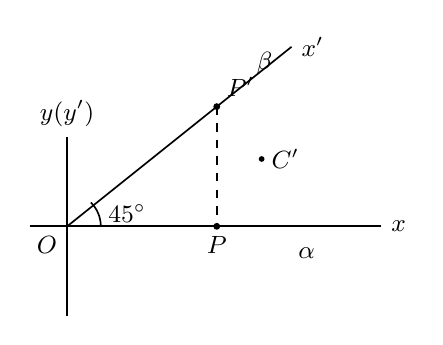
\begin{tikzpicture}[>=stealth, semithick, font=\small, scale=0.95]
  % α 平面（水平）
  \draw (-0.5,0) -- (4.2,0) node[right] {$x$};
  \draw (0,-1.2) -- (0,1.2) node[above] {$y(y')$};
  \node[below left] at (0,0) {$O$};
  \node[below] at (3.2,-0.15) {$\alpha$};
  % β 平面（斜向上 45°）
  \draw (0,0) -- (3.0,2.4) node[right] {$x'$};
  \node[above right] at (2.4,1.9) {$\beta$};
  \draw[dashed] (2.0,1.6) -- (2.0,0) node[below] {$P$};
  \fill (2.0,1.6) circle (1.3pt) node[above right] {$P'$};
  \fill (2.0,0) circle (1.3pt);
  \draw (0.45,0) arc (0:45:0.45) node[midway, right] {$45^\circ$};
  \fill (2.6,0.9) circle (1.1pt) node[right] {$C'$};
\end{tikzpicture}
